%%% wien2wannier/doc/wien2wannier_userguide.tex     %%%
%%%                                                 %%%
%%% Copyright 2009-2012 Philipp Wissgott, Jan Kuneš %%%
%%%           2012-2016 Elias Assmann               %%%

%%% shared-files/header.tex
%%%
%%%    Header for wien2wannier and woptic UGs.
%%%

\documentclass[
   a4paper,
   oneside,
%   twoside,
%   draft
]{wien}
\usepackage[utf8]{inputenc}
\usepackage[osf,sc,slantedGreek]{mathpazo}
\linespread{1.05}
\usepackage[scaled=1.05]{zlmtt}
\usepackage[T1]{fontenc}
\usepackage[protrusion=true,
            expansion=true,
            auto=true,
%            kerning=true,
            spacing=true,
            tracking=false]
           {microtype}

\usepackage{amsmath, amssymb, graphicx, alphabeta, braket, titlepic,
  xspace, minitoc, longtable, siunitx, fancyvrb, enumitem, tabu,
  upgreek, placeins, maybemath, xcolor}

\usepackage[breaklinks,colorlinks,
            linkcolor=black,
            citecolor=black,
            urlcolor=black,
            ]{hyperref}

% \include{texdefine}
\addtolength{\textwidth}{2.5cm}
\addtolength{\oddsidemargin}{-1cm}
\addtolength{\evensidemargin}{-1.6cm}

\newcommand*\name  [1]{\textsc{#1}}
\newcommand*\file  [1]{\texttt{#1}}
\newcommand*\fileit[1]{\texttt{\textit{#1}}}
\newcommand*\code  [1]{\texttt{#1}}
\newcommand*\codeit[1]{\texttt{\textit{#1}}}
% for defaults and the like
\newcommand*\rem   [1]{\textit{\liningnums{#1}}}
\newcommand*\usgrem[1]{\textit{\textrm{#1}}}

\newcommand{\liningnums}[1]{%
  {\fontfamily{pplx}\selectfont #1}}

% lining numbers should go with uppercase
\let\tmp\MakeUppercase
\renewcommand\MakeUppercase[1]{\fontfamily{pplx}\selectfont \tmp{#1}}

\newcommand\MyTOC{
  {
    \linespread{1.1}
    \tableofcontents
  }
}

\newcommand*{\abbrev}[1]{\textsc{#1}}
\newcommand*{\Abbrev}[1]{
  \expandafter\newcommand\csname#1\endcsname{\abbrev{#1}\xspace}
}

\Abbrev{cgs}
\Abbrev{dos}
\Abbrev{soc}
\Abbrev{dft}
\Abbrev{Dft}
\Abbrev{mlwf}
\Abbrev{Mlwf}
\Abbrev{lapw}
\Abbrev{Lapw}
\Abbrev{dmft}
\Abbrev{Dmft}
\Abbrev{uc}
\Abbrev{bz}
\Abbrev{wf}
\newcommand*\wfs{\wf{}s\xspace}

\newcommand*\listnote{%
  This file is read using Fortran list-oriented reads, i.e., items are
  separated by white space.%
}

\newcommand\ProgName[2][]{
  \def\myarg{#1}
  \ifx\empty\myarg
     \ProgNameII{#2}{#2}
  \else
     \ProgNameII{#1}{#2}
  \fi
}
\newcommand\ProgNameII[2]{
  \expandafter\newcommand\csname#2\endcsname{%
    \hyperref[sec:#2]{\file{#1}}%
    \xspace%
  }
  \expandafter\newcommand\csname#2Hd\endcsname{%
    \texttt{#1}%
    \xspace%
  }
}

\newcommand\ProgSec[2][]{
  \def\myarg{#1}
  \ifx\empty\myarg
     \def\separator{}
  \else
     \def\separator{---}
  \fi
  \section[\csname#2Hd\endcsname{} \separator{} #1]
  {\csname#2Hd\endcsname{} \separator{} #1}
  \label{sec:#2}
}

\newcommand*\siunits {\abbrev{si}\xspace}

\newcommand*\case    {\texttt{\itshape case}\xspace}
\newcommand*\deffile {\texttt{\itshape def}\xspace}

\newcommand*\wtow   {\href{http://wien2wannier.github.io/}{\textsc{wien2wannier}}\xspace}
\newcommand*\Wtow   {\href{http://wien2wannier.github.io/}{\textsc{Wien2Wannier}}\xspace}
\newcommand*\woptic {\href{http://woptic.github.io/}{\textsc{woptic}}\xspace}
\newcommand*\Woptic {\href{http://woptic.github.io/}{\textsc{Woptic}}\xspace}
\newcommand*\wien   {\href{http://www.wien2k.at}{\textsc{Wien}2k}\xspace}
\newcommand*\Wien   {\href{http://www.wien2k.at}{\textsc{Wien}2k}\xspace}
\newcommand*\wannier{\href{http://www.wannier.org}{\textsc{wannier90}}\xspace}
\newcommand*\Wannier{\href{http://www.wannier.org}{\textsc{Wannier90}}\xspace}
\newcommand*\xcrys  {\href{http://www.xcrysden.org}{XCrySDen}\xspace}
\newcommand*\vesta  {\href{http://jp-minerals.org/vesta/en/}{\textsc{vesta}}\xspace}
\newcommand*\Vesta  {\href{http://jp-minerals.org/vesta/en/}{\textsc{Vesta}}\xspace}
\newcommand*\gnuplot{\href{http://www.gnuplot.info}{gnuplot}\xspace}

\DeclareMathOperator{\tr}{tr}
\DeclareMathOperator{\sgn}{sgn}
\renewcommand*\Re{\mathop{\operatorname{Re}}}

\newcommand*\dd      {\text{d}}
\newcommand*\ii      {\text{i}}
\newcommand*\ee      {\text{e}}

\newcommand{\mb}{\boldsymbol}

%%%% Including template files %%%%
%%%% User code must set \TemplateDir
\newcommand*\FancyVerbStopString{} % empty line ends template inclusion

%%% begin deep magic %%%
\expandafter\def\expandafter\setCatCode\expandafter{
  \catcode35 = 13 % # = active
}
\expandafter\def\expandafter\resetCatCode\expandafter{
  \catcode35 =  6 % # = argument
}
\setCatCode
\def#{\color{gray}\itshape\char35}
\resetCatCode
\newcommand{\Template}[2][]{%
  \\[\baselineskip]
  \begin{minipage}{\linewidth}
    \VerbatimInput[%
    codes={ \setCatCode },
    label={%
      \raisebox{-.5\height}{\case.#2}%
    },
    frame=lines, framesep=3mm,
    numbers=left,
    #1
    ]{\TemplateDir/case.#2}
  \end{minipage}
  \\[\baselineskip]
}
%%% end deep magic %%%

\newenvironment{usage}{%
  \list{}{
    \leftmargin    .5\parindent
    \listparindent 0em
    \itemindent    \listparindent
    \linespread{1.1}
  }
  \item\relax\ttfamily%
}{\endlist}

\newlist{options}{description}{1}
\setlist[options]{
  font=\ttfamily, itemsep=0em,
  labelindent=.5\parindent, leftmargin=!, labelsep=1em
}

\newlist{linesI}{enumerate}{1}
\setlist[linesI]{
  font=\bfseries,
  label={line \arabic*}
}

\newenvironment{lines}{%
  \begin{linesI}%
    \newcommand*\T[1]{\texttt{\textit{##1}}}
    \newcommand*\U[1]{\si{##1}}
    \newenvironment{flin}[3][V]{%
      \newcolumntype V {>{\ttfamily}l}
      \newcolumntype T {>{\ttfamily\itshape}l}
      \newcolumntype U {s}
      \def\argIII{##3}
      \ifx\empty\argIII
      \else
        \def\argIII{ --- ##3}
      \fi
      \item \code{##2}\argIII
      \vskip-.5\baselineskip    % longtabu produces an inordinately
                                % large separation
      \begin{longtabu} to \linewidth { V ##1 X}
    }{%
      \end{longtabu}%
    }%
    % \newcommand{\flinbrk}{% — does not work
    %   \endtabu\endgroup
    %   \begingroup\tabu to \linewidth { *2{ >{\ttfamily}l } X}%
    % }%
  }{%
  \end{linesI}%
}

\setcounter{minitocdepth}{1}
\setcounter{secnumdepth}{1}
\setcounter{tocdepth}{1}
\dominitoc


%%% Local Variables: 
%%% mode: latex
%%% End: 



\newcommand\TemplateDir{../SRC_templates/}

\newcommand\wienroot{\file{\$WIENROOT}\xspace}

\ProgName[w2w]            {wiiw}
\ProgName[wannier90.x]    {wannierx}
\ProgName                 {wplot}
\ProgName[prepare\_w2wdir]{prepwiiw}
\ProgName[init\_w2w]      {initwiiw}
\ProgName                 {findbands}
\ProgName[write\_inwf]    {writeinwf}
\ProgName[write\_win]     {writewin}
\ProgName[wannier90]      {xwannier}
\ProgName[w2waddsp]       {wiiwaddsp}
\ProgName[write\_inwplot] {writeinwplot}
\ProgName[wplot2xsf]      {wplottoxsf}
\ProgName                 {convham}
\ProgName                 {shifteig}
\ProgName                 {rephase}
\ProgName                 {joinvec}
\ProgName[write\_insp]    {writeinsp}

\author{\name{Elias Assmann} \and \name{Jan Kune\v{s}} \and
  \name{Philipp Wissgott}}
\newcommand*\tit{\texorpdfstring{\Wtow}{Wien2Wannier} 2.0 User's
  Guide}
\newcommand*\subtit{From linearized augmented plane waves to maximally
  localized Wannier functions}
\title{\tit\\[1em]\large\mbox{\it \subtit.}}
\titlepic{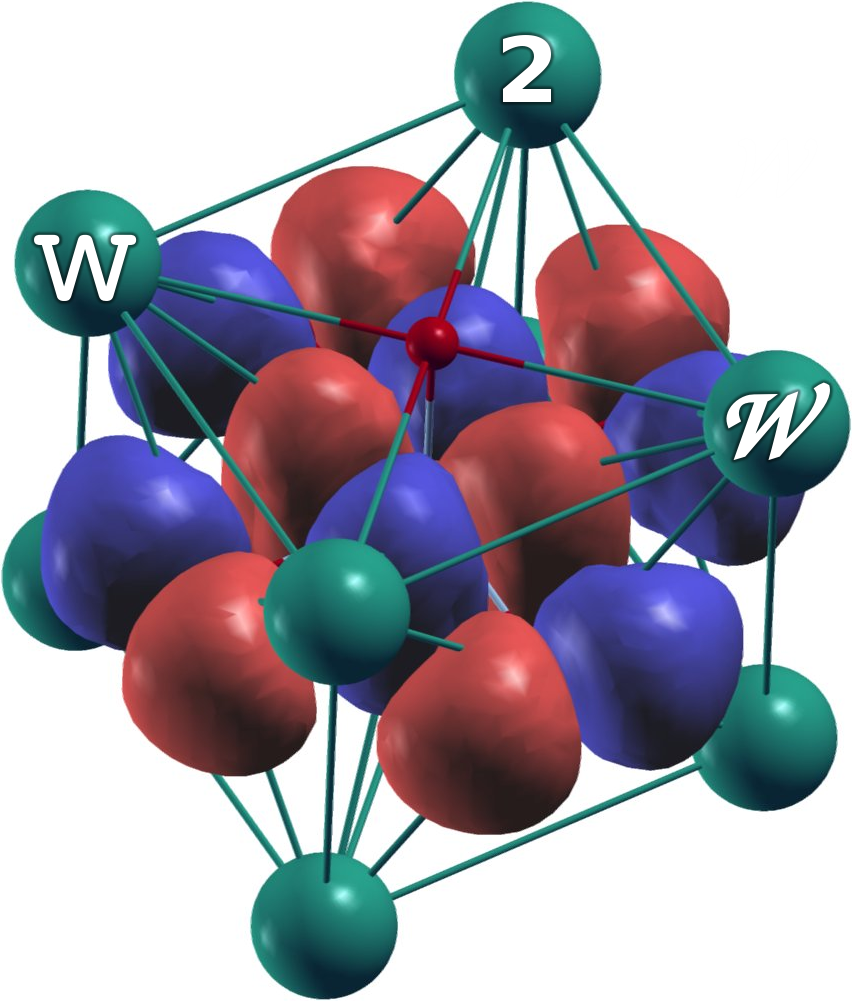
\includegraphics[width=10 cm]{w2w_pic}}

\hypersetup{
  pdftitle={\tit},
  pdfauthor={E. Assmann, J. Kuneš,  and P. Wissgott},
  pdfsubject={\subtit},
}

\begin{document}

\frontmatter
\maketitle

\chapter*{Introduction}
\label{sec:introduction}


In the solid state theorist's tool kit, algorithms based on density
functional theory~(\dft) represent the backbone applications.  One of
the more popular codes available is the \wien
package~\cite{wien2k_orig,wien2k}.  It is based on dividing the real
space unit cell into ``muffin-tin'' spheres centered on the ionic
cores and an interstitial region.  On the former, basis function with
more or less atomic features are employed, while on the latter plain
waves are used.  The combined basis functions are called (linearized)
augmented plane waves (\lapw).

While in \wien a k-space representation of wave functions is
convenient, there are many applications where a real-space picture is
preferable: Determining transport properties~(hopping parameters),
visualization, and, especially, in codes relying on local orbital
basis functions such as dynamical mean-field theory
(\dmft~\cite{dmft}). One way to change to a real space representation
is a Fourier transform of the Bloch states $\psi_{n\mb{k}}(\mb{r})$
from the \dft calculation, yielding
%
\begin{gather*}
  w_{m\mb{R}}(\mb{r})=
  \frac{V}{(2\pi)^3}
  \int_{BZ} dk\ \ee^{-\ii\mb{k}\cdot\mb{R}}
  \left(\sum_nU^{(\mb{k})}_{nm}
    \psi_{n\mb{k}}(\mb{r})\right).
\end{gather*}
%
The resulting functions $w_{m\mb{R}}(\mb{r})$, parametrized by a
direct lattice vector $\mb{R}$, are called Wannier functions
(\wf). Due to the additional phase factors $U^{(\mb{k})}_{nm}$, which
all lead to valid Wannier functions, there is considerable ambiguity
in the choice of the real space basis set.  This can be overcome by
choosing Wannier orbitals $w_{m\mb{R}}(\mb{r})$ with minimal
real-space extent (spread $\langle\Delta \mb{r}^2\rangle$).  These are
known as maximally localized Wannier functions~(\mlwf). A popular
program to compute the \mlwf for a given set of Bloch functions is
\wannier~\cite{wannier90_orig,wannier90}.

Unfortunately, the application of \wannier to the \lapw basis set of
\wien is not as straightforward as for a pure plane wave basis.  In
this guide, we describe the package \wtow which provides an interface
between \wien and \wannier.  In any scientific publications arising
from the use of \wtow, we ask that you cite Ref.~\cite{w2w}.
%
\begin{quote}
  \href{http://www.sciencedirect.com/science/article/pii/S0010465510002948}{
    \name{J. Kune\v{s}, R. Arita, P. Wissgott, A.Toschi, H. Ikeda,}
    and \name{K. Held},\\
    Comput. Phys. Commun. 181, 1888 (2010),
  }
  \href{http://arxiv.org/abs/1004.3934}{arXiv:1004.3934}
\end{quote}
%
to acknowledge your use of our code.  When using \wannier, you should
cite Ref.~\cite{wannier90_orig}
%
\begin{quote}
  \href{http://www.sciencedirect.com/science/article/pii/S0010465507004936}{
    \name{A.A. Mostofi, J.R. Yates, Y.-S. Lee, I. Souza, D. Vanderbilt,}
    and \name{N. Marzari},\\
    Comput. Phys. Commun. 178, 685 (2008),
  }
  \href{http://arxiv.org/abs/0708.0650}{arXiv:0708.0650}
\end{quote}
%
independently of \wtow (cf.~\wannier user's guide \cite{wannier90}).

\paragraph{Acknowledgment}
%
Many thanks to Karsten Held, Peter Blaha, Karlheinz Schwarz, Nikolaus
Frohner, Philipp Hansmann, Nico Parragh and Giorgio Sangiovanni.


\tableofcontents
\listoftodos

\mainmatter


\chapter{Quickstart}
\label{sec:quickstart}
\minitoc

This section outlines the procedure for a ``standard'' \wtow
calculation.  A detailed description of the individual programs can be
found in Section~\ref{sec:detaileddescription}.  For a quick
reference, see the plain-text file \file{CHEATSHEET}.


\section{Preparatory steps}
\label{sec:quickstart_prep}

Before running \wtow, one needs a converged \wien calculation.
Additionally, during the setup for \wtow, the bands which are to be
taken into account will have to be specified, and the main character
(e.g., $d$ bands on atom 2) of these bands should be known.

To obtain this information, a combination of partial DOS and
bandstructure, or a ``band character'' plot is often expedient
(e.g. \file{spaghetti}'s ``fat bands'' option, or
\file{SpaghettiPrimavera} and \file{prima.py}, available in the
\href{http://www.wien2k.at/reg_user/unsupported/}{\textit{unsupported
    software}} section of the \wien website).


\subsection{Copy Required Files}

As a ``zeroth'' step before a Wannier projection, it is recommended to
use the script
\begin{usage}
  \prepwiiw \textit{subdir}
\end{usage}
to create the subdirectory \file{\textit{subdir}} where the rest of
the workflow will take place. Thus, one \wien calculation can be the
starting point of several \wtow runs.


\section{Interface \& Wannierization}
\label{sec:quitckstart_main}

\subsection{Write Input Files}
\label{sec:init}

The script \initwiiw takes the following steps:
%
\begin{description}
\item[\file{x kgen -fbz}] generates the non-symmetrized k-mesh that
  \wannier requires.  The density of the mesh influences the quality
  of localization and visualization of the Wannier functions.  Remark:
  The interface was only tested with unshifted k-meshes.
\item[\file{x \findbands}] looks in \file{\case.output1} for bands in a
  given energy range $[E_\text{min}, E_\text{max}]$, and outputs the
  corresponding band indices $b_\text{min}, b_\text{max}$.  To choose
  the energy window of interest, consult a (p)DOS and/or band
  structure plot.
\item[\writeinwf] writes the main input file \file{\case.inwf} for the
  interface.  The band indices $b_\text{min}$, $b_\text{max}$ have to
  be specified, and initial projections $A_{mn}$ may be given in terms
  of atomic sites and appropriate spherical harmonics.
\item[\writewin] writes the input file for \wannierx, \file{\case.win},
  on the basis of \file{\case.inwf} and other files.
\item[\file{x \xwannier{} -pp}] reads the k-mesh in \file{\case.win} and
  writes a list of nearest-neighbor k-points to \file{\case.nnkp}.
\end{description}


\subsection{Run Interface}
After running \initwiiw, one can proceed:
\begin{description}
\item[\file{x lapw1}] before the actual interface run, the
  eigenvectors and eigenvalues for the new (non-symmetrized) k-mesh
  have to be computed.
\item[\file{x w2w}] computes the overlaps $M_{mn}$, initial
  projections $A_{mn}$ and eigenvalues $E_n$, and writes them to
  \file{\case.mmn}, \file{\case.amn}, and \file{\case.eig}.
\end{description}


\subsection{Run Wannierization}
Finally,
\begin{description}
\item[\file{x \xwannier}] computes the $U(\mb k)$ by maximum
  localization.  Output is stored in \file{\case.wout}. The Wannier
  orbitals should be converged to a spread which is usually smaller
  than the unit cell of the structure.
 \end{description}


\section{Verification \& Postprocessing}
\label{sec:quickstart_post}

After a successful \wannier run, one should check if the centers and
spreads of the Wannier functions (printed in \file{\case.wout}) are
sensible.  Another important consistency check is to compare the
Wannier-interpolated bandstructure to the one computed by \wien.
\Wtow also provides programs to create a real-space plot of the
Wannier functions.

\subsection{Compare Bandstructures}
With the option \file{hr\_plot=T}, \wannier writes a bandstructure
derived from the Wannier-inter\-po\-la\-ted Hamiltonian $H(\mb k)$ to
\file{\case{}\_band.dat}.  To compare this to the bandstructure
computed by \file{spaghetti}, e.g.\ in \file{gnuplot}, use the command
(including a conversion from Bohr$^{-1}$ to \AA{}ng\-str\"om$^{-1}$)
\begin{usage}
  p '\case.spaghetti\_ene' u (\$4/0.53):5, '\case{}\_band.dat' w l
\end{usage}

\subsection{Plot Wannier Functions}
\begin{description}
\item[\writeinwplot] asks for a real-space grid on which the
  Wannier functions should be plotted, and writes
  \file{\case.inwplot}.
\item[\file{x wplot -wf \textit{m}}] evaluates Wannier function number
  $m$ on the real-space grid, and writes the density $|w_m(\mb r)|^2$
  to \file{\case{}\_\textit{m}.psink} and the phase $\arg w_m(\mb r)$
  to \file{\case{}\_\textit{m}.psiarg}.
\item [\wplottoxsf] converts all \file{\case{}*.psink} plus
  \file{\case{}*.psiarg} files in the directory to \file{xsf} files
  which can be opened by \xcrys.
\item [\file{xcrysden --xsf \case{}\_\textit{m}.xsf.gz}] ; pick
  ``Tools $\rightarrow$ Data Grid'' from the menu and press OK. In the
  isosurface controls window choose an appropriate isovalue, e.g. 0.1,
  and check the ``Render +/- isovalue'' box.
\end{description}


\chapter{Detailed description}
\label{sec:detaileddescription}
\minitoc

This section lists the programs included in \wtow, along with brief
descriptions and usage summaries.  All programs have online help
(\file{-h}), which may be more complete than the material here.

Programs that are described here include: the ``main'' \wtow programs
\wiiw and \wplot; several utility programs used in a typical \wtow
run; and some programs that are needed in special cases, or grew out
of \wtow development and are provided here in the hope that they will
be useful, even if they are not needed in the context of \wtow.


\ProgSec[compute overlaps]{wiiw}

This is the main program of the interface which provides the files
\file{\case.mmn}, \file{\case.amn} and \file{\case.eig} for \wannier
given the output of a \wien run (most importantly,
\file{\case.vector}).  \wiiw is based on \file{lapwdm}, since the main
task, for the computation of the overlap matrices
\begin{eqnarray}
\label{eq:mmn}
M_{mn}^{(\mb{k},\mb{b})}&=&\langle
\psi_{m\mb{k}}|\ee^{-\ii\mb{b}\cdot\mb{r}}|\psi_{n\mb{k}+\mb{b}}
\rangle
\label{eq:mmn2}
\end{eqnarray}
that are stored in \file{\case.mmn}, is to determine the basis
functions $\psi_{n\mb k}(r)$ in the entire unit cell (using
appropriate boundary conditions on the muffin-tin spheres).

In addition to standard \wien files, a file \file{\case.nnkp} is
required which defines the ${\mb b}$ vectors for each ${\mb k}$ in
Eq.~(\ref{eq:mmn2}).  \wannierx delivers this file when called with
the flag \file{-pp}.

\subsection{Execution}

The program \wiiw is executed by invoking the command:
%
\begin{usage}
  x w2w [-c -up|-dn -so -p] |
  \\
  w2w w2w.def [\#proc]
  |
  w2wc w2w.def [\#proc]
\end{usage}

While \wiiw itself is not parallelized, like \file{x lapw2 -qtl}, it
accepts a \file{-p} switch (or \file{\#proc}) to read parallel
\file{vector} and \file{energy} files.

With spin-orbit coupling (\file{-so}), \wiiw must be called separately
for \file{-up} and \file{-dn}, resulting in\linebreak[4]
\file{\case.mmn\{up,dn\}}, \file{\case.amn\{up,dn\}}, and
\file{\case.eig\{up,dn\}}.  In a second step, the $M_{mn}$ and
$A_{mn}$ must be added (and the eigenvalues copied) to produce
\file{\case.mmn}, \file{\case.amn}, and \file{\case.eig}, on which
\wannier may be run.  This step is done by the program \wiiwaddsp,
which is automatically invoked by \file{x \xwannier{} -so}.


\subsection{Input}

A sample input file for \wtow is given below. It can be generated
using \writeinwf.
%
\Template{inwf}
%
\listnote

\begin{lines}
  \begin{flin}{mode}{what to calculate}
    mode & Amn & Only determine the initial orbital projections
                 \file{\case.amn}\\
         & Mmn & Only determine the overlap matrices \file{\case.mmn}\\
         & both& Determine both the initial orbital projections and the
          overlap matrices
 \end{flin}

 \begin{flin}[T]{Blo, Bhi}{band window}
   Blo, Bhi & int & the minimal and maximal Bloch band from the vector
                    file to be taken into
                    account, determining the lower edge of the (outer) energy
                    window
 \end{flin}

 \begin{flin}[T]{LJmax, Nproj}{}
   LJmax & int & the number of terms which are used in the spherical
                 harmonics expansion to approximate $\exp(-\ii \mb k\mb
                 b)$, usually 3--4 is sufficient.\\
   Nproj & int & the number of target Wannier functions
 \end{flin}

 \begin{flin}[T]{Nterm}{number of terms \rem{(\code{Nproj} times)}}
   Nent & int & the number of $Y_\ell^m$ terms (lines to follow for
                this initial projection
 \end{flin}

 \begin{flin}[T]{Iat, l, m, Re, Im}{$Y_\ell^m$ term \rem{(\code{Nterm}
       times)}}
   Iat   & int & the atom where the entry is centered\\
   l, m  & int & the orbital and magnetic quantum numbers $\ell$ and
                 $m$ for this entry\\
   Re, Im& real& the complex coefficient multiplying $Y_\ell^m$
 \end{flin}
\end{lines}

If initial projections are given, there must be \code{Nproj} blocks
\textbf{l.~4+5}, one for each initial projection.  Within each block,
write \code{Nterm} lines \textbf{l.~5}, one for each $Y_\ell^m$ term.
Otherwise, if \code{mode} is \code{Mmn}, the initial projections can
be omitted.

\paragraph{Note} The initial projections (\textbf{l.~5}) generated by
\writeinwf are normalized.  For non-normalized initial projections (as
in the template), the extra factor will be included in
\file{\case.amn}, but neutralized by the orthonormalization step in
\wannier.


\ProgSec[Wannier function plotter]{wplot}

\wplot evaluates the Wannier functions on a real-space grid.  It reads
the transformation matrices $U(\mb k)$ from the file \file{\case.chk}
written by \wannierx and thereby constructs the Wannier functions from
the original \wien Bloch states.

\subsection{Execution}

The program \wplot is executed by invoking the command:
%
\begin{usage}
  x wplot [-up|-dn -c -so -p -wf \textit{m}]   |
  \\
  wplot  \deffile [\textit{m} [\#proc]] |
  wplotc \deffile [\textit{m} [\#proc]]
\end{usage}
%
\wplot is not parallelized, but accepts a \file{-p} switch (or
\file{\#proc}) to read parallel \file{vector} files.  Moreover, as a
crude form of parallelization, one can run several \wplot instances in
the same directory in parallel without interference (e.g. to plot
several Wannier functions on fine grids).

The input file contains the index of the Wannier orbital to be
plotted; \file{\textit{m}} above overrides this.  Output goes to
\file{\case{}\_\textit{m}.psink} ($|w(\mb r)|^2$) and
\file{\case{}\_\textit{m}.psiarg} ($\arg w(\mb r)$).

\subsection{Input}

\wplot is based on \file{lapw7} and shares the general structure of
the input file.  A sample input file for \file{wplot} is given below.
It can be generated via \writeinwplot, or adapted from the template in
\file{\wienroot/SRC\_templates}.
%
\Template{inwplot}
%

\begin{lines}
  \begin{flin}{mode, flag \rem{format(A3, A1)}}{}
  mode & 3D  & a regular grid will be specified\\
       & ANY & read arbitrary grid from \file{\case.grid}\\
  flag & O,N & when \code{mode =  3D}: check for orthogonality or not\\
       & C,F & when \code{mode = ANY}: cartesian or fractional coordinates
  \end{flin}
%
  If \code{mode=3D} and \code{flag=O}, grid axes will be checked for
  pairwise orthogonality; set \code{flag=N} for nonorthogonal axes.
  If \code{mode=ANY} and \code{flag=C}, the grid points in
  \file{\case.grid} are in cartesian coordinates (3 reals per line);
  if \code{flag=F}, they are in fractional coordinates (3 numbers and
  divisor).

  \begin{flin}[T]{ix, iy, iz, idv \rem{(free format)}}{grid origin
      \rem{(\code{mode=3D})}}
    ix,iy,iz,idv & int& Coordinates of the origin of the grid, where x=ix/idv
                        etc. in units of the \emph{conventional}
                        lattice vectors
  \end{flin}

  \begin{flin}[T]{ix, iy, iz, idv \rem{(free format)}}{axis end-point
      \rem{(\code{mode=3D}; 3 times)}}
    ix, iy, iz, idv & int & Coordinates of the end points of each grid axis
  \end{flin}

  \begin{flin}[T]{nx, ny, nz \rem{(free format)}}{mesh size}
    nx,ny,nz & int & number of mesh points in each direction
                     \rem{(\code{mode=3D})}\\
    npt      & int & total number of mesh points \rem{(\code{mode=ANY})}
  \end{flin}

  If \code{mode=3D}, give \textbf{l.~3} 3 times, once for each
  direction; if \code{mode=ANY}, omit \textbf{l.~2+3} and give the
  total number of points to be read on \textbf{l.~4}.

  \begin{flin}{post \rem{format(A3)}}{post-processing option}
    post & DEP & ``dephasing'': each wave function is multiplied by a
                 complex phase factor to align it~(as far as possible)
                 to the real axis\\
         & NO  & No post-processing
  \end{flin}

  \begin{flin}{unit, whpsi \rem{(free format)}}{}
    unit & ANG      & Ångström\\
         & AU$|$ATU & Atomic units\\
    whpsi& LARGE & the large relativistic component for each wave
                   functions is evaluated\\
         & SMALL & small relativistic component
  \end{flin}

  \begin{flin}[T]{iwan, wfrot \rem{(free format)}}{\wf index, apply \wf
      rotation?}
    iwan & int & index of the \wf to be plotted, unless overridden on
                 command line\\
    wfrot& logical & read unitary matrix from \file{\case.wfrot} and
                     apply before plotting
  \end{flin}
\end{lines}

Finding the right window for plotting can be tricky.  \Wannier often
yields orbitals that are not centered in the home unit cell;
\wplottoxsf can shift them later on, but in \wplot one has to ``hit''
the orbitals as given by \wannier (see section ``Final State'' in
\file{\case.wout}).  Therefore, it is recommended to start with a
coarse grid (for instance $10\times10\times10$), make sure the window
is correct, and only then start a calculation with a finer grid.

The option \file{wfrot} asks \wplot to read a $(N_\wf \times N_\wf)$
matrix from \file{\case.wfrot}, which is applied to the \wfs before
plotting.  This is useful for some post-processing applications, where
a rotation in the Wannier subspace is desired.


\ProgSec[copy required files]{prepwiiw}

A \wien computation can be the starting point for various runs of
\wtow. This script creates a new subfolder of a \wien directory and is
invoked by
%
\begin{usage}
  \prepwiiw \textit{subdir}
\end{usage}
%
where \file{subdir} is the name of the subdirectory to be created.


\ProgSec[prepare \wtow input files]{initwiiw}

This script guides the user through the initialization of \wtow phase
as described in Section \ref{sec:init}.
%
\begin{usage}
  \initwiiw [-up|-dn] [-b \textit{options}]
\end{usage}
%
In batch mode (\file{-b}), further options are available instead of
interactive input.


\ProgSec[get band indices inside energy interval]{findbands}

This program reads \file{\case.output1} to identify the bands which
lie within a certain energy window. The program \findbands is
executed by issuing the command:
%
\begin{usage}
  x \findbands \textit{window} [-up|-dn -so -hf -efermi EF]
  |
  \\
  \findbands \deffile
\end{usage}
%
\file{\textit{window}} may be given as \file{-emin e -emax E} or
\file{-all e E}.  The energies are in eV with $E_\text F = 0$.  The
Fermi energy is read from \file{\case.fermi} (written by \prepwiiw)
unless given as \file{-efermi} (in Ry).

The output is given in \file{\case.outputfind} and consists of the
bands in the interval at each k-point, as well as which bands are
contained in the interval across all k-points, and which bands cross
the interval at any k-point.


\ProgSec[prepare input file for \wiiw]{writeinwf}

This program prepares the main input file \file{\case.inwf} for
\wiiw.  It is executed by invoking the command
%
\begin{usage}
  \writeinwf \usgrem{(interactive)} |
  \\
  \writeinwf{} -bands Nmin Nmax PROJ [PROJ ...]
  \usgrem{(noninteractive)}
\end{usage}
%
It will ask (in interactive mode) for a range of bands, which are all
the bands to be taken into account by \wiiw (including those for
disentanglement).  Then, it will ask for ``projection specifications''
\file{PROJ = SITE:ORB[:ZAXIS[:XAXIS]]}, which consist of colon-
separated parts naming an atomic site, an orbital, and, optionally,
rotated $z$- and $x$-axes\footnote{\writeinwf uses the method of
  Ref.~\cite{ylmrot} to rotate the spherical harmonics.}.  Please see
\file{write\_inwf -h} and \file{write\_inwf -H axes/sites/orbitals}
for further information on these.  Interactively, you can also use tab
completion to discover input options and command line history to
recall past inputs.

The program will keep asking for projections until it has accumulated
as many projections as bands were specified.  However, one can stop
early by pressing \file{Ctrl-D} (EOF); in this case, there will be
fewer Wannier functions than bands (disentanglement).


\ProgSec[prepare input file for \wannierx]{writewin}

This program reads \file{\case.inwf}, \file{\case.klist}, and some
other files, and produces \file{\case.win}, the input file for
\wannierx.  It is executed by invoking the command
%
\begin{usage}
  \writewin [-fresh]
\end{usage}

If \file{\case.win} already exists, \file{write\_win} updates it.
Otherwise (or if \file{-fresh} is given), the template in
\file{\wienroot/SRC\_templates} is used.


\ProgSec[wrapper for \wannierxHd]{xwannier}

A wrapper script for \wannierx is provided to take care of spin
polarization and spin-orbit coupling.  In the context of \wtow,
\wannierx is executed by invoking the command
%
\begin{usage}
  x \xwannier [-up|-dn|-so|-pp] |
  \xwannier [-up|-dn|-so|-pp]
\end{usage}
%
The wrapper script must be able to find the executable \wannierx,
i.e. you have to either have it in your \file{\$PATH}, or edit the
script \file{wannier90\_lapw} to provide the location.

With \file{-pp}, \wannierx will produce \file{\case.nnkp}; with
\file{-so}, \wiiwaddsp will be called to add the spin channels
together before running \wannierx.

Extensive diagnostic output goes to \file{\case.wout}, error messages
to \file{\case.werr}; the full results (in particular the $U(\mb k$)
matrices) are stored in the binary file \file{\case.chk}.


\ProgSec[add spin directions for SOC]{wiiwaddsp}

In calculations including spin-orbit coupling (\soc), \wannier has to
be invoked on \file{\case.mmn} and \file{\case.amn} files which
contain the sum of the overlaps / projections for the two spin
channels.  (This procedure is needed also for non-spin-polarized
cases, cf.~Section~\ref{sec:wiiw}.)  To this end, \file{w2waddsp}
reads \file{\case.mmn\{up,dn\}}, \file{\case.amn\{up,dn\}} and writes
\file{\case.mmn}, \file{\case.amn}.

There is usually no need to call this program manually, it is run by
\file{x \xwannier{} -so}.  If needed, it is executed by invoking the
command
%
\begin{usage}
  x \wiiwaddsp |
  \wiiwaddsp \deffile
\end{usage}
%
after running \file{x \wiiw -up} and \file{-dn}.


\ProgSec[prepare input file for \wplot]{writeinwplot}

This program may help in preparing the input file for \wplot.
(Alternatively, copy the template from
\file{\wienroot/SRC\_templates}.)  It is executed by invoking the
command
%
\begin{usage}
  \writeinwplot \case
\end{usage}


\ProgSec[convert \wplot output to \file{xsf} format]{wplottoxsf}

This program converts the files \file{\case{}\_\textit{m}.psink} and
\file{\case{}\_\textit{m}.psiarg} produced by \wplot to files
\file{\case{}\_\textit{m}.xsf} which can be opened, e.g., in
\xcrys \cite{xcrys} or \vesta \cite{vesta}.

Note that only real data can be represented in the \file{xsf} file.
Therefore, $|w(\mb r)|^2 \sgn \Re w(\mb r)$ is saved by default.  (In
most cases the Wannier functions are real anyway.)

\file{wplot2xsf} has a number of options (see \file{wplot2xsf -h}),
but usually it is executed by invoking the command
%
\begin{usage}
  \wplottoxsf [-up|-dn]
\end{usage}
%
If all the required files have their standard names, this will convert
all the plots in the current directory.

By default, \file{wplot2xsf} reads \file{\case{}\_centres.xyz}, and
shifts the Wannier functions so that their centers have the
coordinates given in that file.  If \file{translate\_home\_cell} (and
\file{write\_xyz}) is set in \file{\case.win}, this will result in a
plot where the Wannier centers lie in the ``home'' unit cell.


\ProgSec[Fourier transform Wannier Ham\-il\-to\-ni\-an]{convham}

This program Fourier transforms the \wannier real space Hamiltonian
$H(\mb R)$ (\file{\case{}\_hr.dat}) to its k-space representation $H(\mb
k)$ (\file{\case.ham\_fine}) on the k-points given by
\file{\case.klist}.  In this way, if the real-space Hamiltonian is
sufficiently localized, $H(\mb k)$ may be interpolated to arbitrarily
fine k-grids.  \file{convham} is executed by invoking the command
%
\begin{usage}
  x \convham [-band]
  | \\
  \convham \deffile
\end{usage}

\ProgSec[shift energies in \file{\case.eig}]{shifteig}

to zero in \file{\case.eig}.  If needed, this program can be used to
apply an additional shift by \file{DE} (in eV).  \file{shifteig} is
executed by invoking the command
%
\begin{usage}
  x \shifteig [-up|-dn] -efermi DE |
  \shifteig \deffile DE
\end{usage}


\ProgSec{rephase}

program reads the psiarg files to determine the most probable phases
of all Wannier functions. Then, the input for the interface file
\case.inwf is rewritten in a way that a subsequent run of \wtow and
\wannier leads to real Wannier orbitals~(this does not work in all
cases). The Fortran program \file{rephase} is invoked by the command
%
\begin{usage}
  \rephase \case [-w] [-up/-dn] [-wf=idx\_wann]
\end{usage}
%
where the option -w means that \file{\case.inwf} is automatically
updated~(future wien2wannier runs will then have a higher probability
of producing real Wannier orbitals) and the option -w idx\_wann
indicates that the action is only applied for the Wannier function
\file{idx\_wann}.


\ProgSec[join parallel \file{vector} files]{joinvec}

\file{energy} files from a parallel calculation into one
\file{\case.vector} and one \file{\case.energy}.  It is executed by
invoking the command
%
\begin{usage}
  x \joinvec [-up|-dn -c -so]
\end{usage}
%
All \file{.vector\_*} files are merged into one \file{.vector} file
containing the header of the first file \file{.vector\_1}~(and
correspondingly for the \file{.energy} files).


\ProgSec[write input file for \file{spaghetti}]{writeinsp}

Fermi energy read from \file{\case.scf2} in the input file for
\file{spaghetti}, \file{\case.insp}. It is invoked by
%
\begin{usage}
  \writeinsp [-up/-dn]
\end{usage}


% \chapter{Installation}
% \label{sec:installation}

% This procedure assumes that \wien is unpacked and configured (i.e. you
% have run \file{siteconfig}) in a
% directory \wienroot.

% \section{\wtow}
% \label{sec:install:wien2wannier}

% Get the source from
% \url{http://www.ifp.tuwien.ac.at/forschung/arbeitsgruppen/cms/software-download/wien2wannier/}
% and unpack,
% %
% \begin{verbatim}
%    $ tar -xvf wien2wannier-X.Y.tar.gz
% \end{verbatim}

% The directory \file{wien2wannier-X.Y/} has been created.  Installation
% instructions are provided in the file \file{INSTALL}.


% \section{\wannier}
% \label{sec:install:wannier90}

% \Wannier can be downloaded from \url{http://wannier.org}.  It should
% be compiled with the same settings as \wtow, because \wplot needs to
% read the binary \file{chk} file.  You can find these settings in
% \file{\wienroot/\{COMPILER,OPTIONS\}}.  Refer to the \wannier
% documentation for furtherinstallation instructions.


\chapter{Getting help}

Online help for all programs can be requested via the option
\code{-h}.  In addition to the pointers below, the \wtow distribution
also includes a file \file{CHEATSHEET}, which concisely summarizes the
usual steps of a calculation.  If this does not help, send questions
relating to the usage of \wtow to the Wien2k mailing list at
\url{http://www.wien2k.at/reg_user/mailing_list/}.  For questions
about \wannier and the \mlwf procedure, there is a mailing list at
\url{http://www.wannier.org/forum.html}.  The \wtow maintainer can be
reached at \url{wien2wannier@ifp.tuwien.ac.at}.


\section{FAQ}

\subsection{How does one choose the initial projections?}
There is no general rule to choose the initial projections which have
to be prepared in the \file{inwf} file. There are, however, some hints
which usually help:
\begin{itemize}
\item In the energy interval of interest, identify the main atoms
  which contribute to the partial DOS. These atoms are usually good
  centers for the initial projections. The character of these atomic
  contributions can also be seen via the partial DOS.
\item A glance at the bandstructure often helps to consider the
  multiplicity of equivalent \wf and to identify certain
  hybridizations.
\end{itemize}

\subsection{The resulting Wannier orbitals are not localized}
Several possible reasons (this list is not complete)
\begin{itemize}
\item choosing non-optimal initial projections
\item the number of k-points is too small
\end{itemize}

\subsection{The bandstructure of \wien and \wannier does not match}
First of all, be sure to take into account the Bohr-Ångström
conversion, e.g., in \file{gnuplot}:
\begin{usage}
  p '\case.spaghetti\_ene' u (\$4/0.53):5, '\case{}\_band.dat' w l
\end{usage}

If the bands themselves differ strongly, then one might have
\begin{itemize}
 \item non-optimal initial projections
 \item too few k-points
 \item chosen the frozen energy window in \wannier in a wrong way.
\end{itemize}

\subsection{When plotting a Wannier orbital in \xcrys I can see nothing}
One possible reason is that the \wf centers are not necessarily in the
home unit cell at $[0\, 0\, 0]$.  The interface programs usually
account for this by translating the \wf to the home cell.  However, the
spatial mesh for \wplot has to be defined with respect to the original
centers which come out of \wannier.  These centers can be found in
\file{\case.wout} file.  Assume the \wf is centered at $[-0.5\, -0.5\,;
-0.5]$ in the basis of conventional unit vectors. Then, appropriate
mesh vectors might be
\begin{Verbatim}
-1 -1 -1 1     #x, y, z, divisor of orig
 0 -1 -1 1     #x, y, z, divisor of x-end
-1  0 -1 1     #x, y, z, divisor of y-end
-1 -1  0 1     #x, y, z, divisor of z-end
\end{Verbatim}

\subsection{My Wannier orbitals are not centered at the home unit
  cell}

It happens quite frequently that a \wf is not centered within the home
unit cell, which is displayed by default by \xcrys. The interface
program \writewin automatically activates the option
\code{translate\_home\_cell} in the \wannier input file. Then,
\wannier should produce a file \file{\case{}\_centres.xyz}, where the
vectors of all \wf are stored which translate the orbital to the home
unit cell. If this file cannot be located by \wplottoxsf or the option
--noshift is activated, no translation is conducted and the \wf appear
centered at their original position.


\begin{thebibliography}{88}
\bibitem{wien2k_orig}
  \name{P. Blaha, K. Schwarz, G.K.H. Madsen, D. Kvasnicka}, and
  \name{J. Luitz.}
  \textit{\Wien, An Augmented Plane Wave + Local Orbitals Program for
    Calculating Crystal Properties.}
  Techn. Universität Wien, Austria, 2001.
  \url{http://www.wien2k.at}.

\bibitem{wien2k}
  \name{P. Blaha, K. Schwarz, G.K.H. Madsen, D. Kvasnicka, J. Luitz.}
  \textit{\Wien User's Guide.}\linebreak[4]
  \url{http://www.wien2k.at/reg_user/textbooks/usersguide.pdf}.

\bibitem{dmft}
  \name{K. Held.}
  \textit{Electronic structure calculations using dynamical mean field
    theory.}
  \href{http://www.tandfonline.com/doi/abs/10.1080/00018730701619647}{%
    Adv. Phys. {\bf 56}, 829-926 (2007).
  }

\bibitem{wannier90_orig}
  \name{A.A. Mostofi, J.R. Yates, Y.-S. Lee, I. Souza, D. Vanderbilt}
  and \name{N. Marzari.}\linebreak[4]
  \textit{\wannier: A tool for obtaining maximally-localized Wannier
    functions.}
  \href{http://www.sciencedirect.com/science/article/pii/S0010465507004936}{%
    Comput. Phys. Commun. \textbf{178}, 685~(2008)
  }

\bibitem{wannier90}
  \name{A.A. Mostofi, J.R. Yates, Y.-S. Lee, I. Souza,
    D. Vanderbilt} and \name{N. Marzari.}\linebreak[4]
  \textit{\Wannier User Guide.}
  \url{http://wannier.org/doc/user_guide.pdf}.

\bibitem{w2w}
  \name{J. Kune\v{s}, R. Arita, P. Wissgott, A.Toschi, H. Ikeda,}
  and \name{K. Held.}
  \textit{\Wtow: From linearized augmented plane waves to maximally
    localized Wannier functions.}
  \href{http://www.sciencedirect.com/science/article/pii/S0010465510002948}{%
    Comput. Phys. Commun. \textbf{181}, 1888~(2010).%
  }

\bibitem{ylmrot}
  \name{Z. Romanowski} and \name{S. Krukowski.}
  \textit{Transformations of complex spherical harmonics under
    rotations.}
  \href{http://iopscience.iop.org/1751-8121/40/50/011}{%
    J. Phys. A: Math. Theor. \textbf{40}, 15071~(2007).%
  }

\bibitem{xcrys}
  \name{A. Kokalj.}
  \textit{Computer graphics and graphical user interfaces as tools in
    simulations of matter at the atomic scale.}
  \href{http://www.sciencedirect.com/science/article/pii/S0927025603001046}{%
    Comput. Mater. Sci., {\bf 28}, 155 (2003).%
  }; \url{http://www.xcrysden.org}.

\bibitem{vesta}
  \name{K. Momma} and \name{F. Izumi.}
  \textit{VESTA \liningnums{3} for three-dimensional visualization of
    crystal, volumetric and morphology data.}
  J. Appl. Cryst. 44, 1272 (2011).
  \url{http://jp-minerals.org/vesta/en/doc.html}.

\end{thebibliography}
\end{document}

%%% Time-stamp: <2016-11-29 22:49:45 ea@archpad>
